% Musterblatt Terme, von Hand gesetzt (Lehrerbefunde 01.10.2026)
% Quelle je Teilaufgabe im Kommentar davor: % <id> = wortgleich aus der
% Bank (Auftrag in den Titel der Hauptnummer gezogen), % GEÄNDERT <id> =
% Zahlen oder Form geändert, % NEU = nicht in der Bank.
% % pruef: … ist die Rechenprobe für pruef.py (Textaufgaben).
% Blattfolge 2, 3, 4, 1 (katalog/terme.md).
\documentclass[11pt]{article}
\usepackage{mathblatt}
\usepackage{multicol}
\blattfuss{Terme}{Muster 2026-10-01}
\raggedright
\makeatletter
% ---------------------------------------------------------------- Satz
% Einheitentitel wie ein Kapitel; neue Seite nur, wenn weniger als ein
% Drittel frei ist
\newcommand{\einheit}[1]{\par\Needspace*{0.33\textheight}\addvspace{16pt}%
  \noindent{\Large\bfseries #1}\par\vspace{1.5mm}%
  \noindent\rule{\textwidth}{0.6pt}\par\nobreak\vspace{2pt}%
  \gappto\mblsg{\lsgeinheit{#1}}}
% Hauptnummer: Titel und Auftrag in einer Zeile. Ohne Option bleibt sie
% auf einer Seite; mit [b] (reine Rechenketten) darf sie zwischen zwei
% Zeilen umbrechen, Titel und die ersten vier Zeilen bleiben zusammen.
\newsavebox{\nrbox}\newlength{\nrhoehe}
\newcommand{\nrtitel}[1]{\noindent\hangindent1.6em\hangafter1%
  \makebox[1.6em][l]{\textbf{\theaufgabe.}}#1\par\vspace{1pt}}
\newenvironment{nr}[2][]{\refstepcounter{aufgabe}\setcounter{teil}{0}%
  \def\nrart{#1}%
  \ifx\nrart\@empty
    \begin{lrbox}{\nrbox}\begin{minipage}[t]{\linewidth}\raggedright
    \setlength{\parskip}{0pt}\nrtitel{#2}%
  \else
    \par\addvspace{11pt}\Needspace*{8\baselineskip}\nrtitel{#2}%
  \fi}%
 {\ifx\nrart\@empty
    \end{minipage}\end{lrbox}%
    \setlength{\nrhoehe}{\dimexpr\ht\nrbox+\dp\nrbox\relax}%
    \par\addvspace{11pt}\Needspace*{\nrhoehe}\noindent\usebox{\nrbox}\par
  \else\par\fi}
% Buchstabe der Teilaufgabe, rechtsbündig in 1,6 em
\newcommand{\teilmarke}{\stepcounter{teil}\makebox[1.6em][r]{\alph{teil})\hspace{0.35em}}}
\newlength{\feldbreite}\setlength{\feldbreite}{4.5cm}
\newcommand{\antwort}{\underline{\hspace{\feldbreite}}}
% Zeilenabstand der Ketten: Schreibhöhe für die Antwort
\newcommand{\zeilenluft}{\par\nobreak\vskip 12pt plus 1pt\relax}
\newcommand{\zeilenluftb}{\par\vskip 12pt plus 1pt\relax}
% Rechenkette: Gleichheitszeichen in einer Flucht (Termspalte so breit
% wie der breiteste Term der Kette), Antwortfeld in der Zeile. Die Zeilen
% werden erst gesammelt und am Ende gesetzt; jede Zeile ist ein eigener
% Absatz. Umbruch nur so, dass auf beiden Seiten mindestens drei Zeilen
% stehen.
\newlength{\kw}\newlength{\kwmax}
\newcounter{kzahl}\newcounter{kzeile}
\newcommand{\kliste}{}
\newcommand{\kmerke}[2]{\settowidth{\kw}{#1}%
  \ifdim\kw>\kwmax\global\kwmax=\kw\fi\stepcounter{kzahl}\gappto\kliste{#2}}
\newcommand{\kstart}[1]{\global\kwmax=0pt\setcounter{kzahl}{0}\setcounter{kzeile}{0}%
  \gdef\kliste{}\setlength{\feldbreite}{#1}}
\newcommand{\kende}{\par\vspace{3pt}\kliste\par}
\newcommand{\kettezeile}[1]{\stepcounter{kzeile}%
  \ifnum\value{kzeile}>1
    \ifnum\value{kzeile}<4 \zeilenluft
    \else\ifnum\numexpr\value{kzahl}-\value{kzeile}\relax<2 \zeilenluft
    \else\zeilenluftb\fi\fi
  \fi
  \noindent#1\par}
\newenvironment{kette}[1][4.5cm]{\kstart{#1}}{\kende}
\newcommand{\rk}[2]{\kmerke{$#1$}{\kettezeile{\teilmarke\lsgm{#2}%
  \makebox[\kwmax][r]{$#1$}\hspace{0.45em}$=$\hspace{0.45em}\antwort}}}
% Termwert: Term, Einsetzung, Feld (Spalten wie die Kette)
\newenvironment{werte}[1][2.6cm]{\kstart{#1}}{\kende}
\newcommand{\rw}[4][4.6cm]{\kmerke{$#2$}{\kettezeile{\teilmarke\lsgm{#4}%
  \makebox[\kwmax][r]{$#2$}\hspace{1.2em}\makebox[#1][l]{für $#3$:}\antwort}}}
% Ohne Feld (Unterstreichen)
\newenvironment{liste}{\kstart{0pt}}{\kende}
\newcommand{\ru}[2]{\kmerke{}{\kettezeile{\teilmarke\lsgt{#2}#1}}}
% Textzeile, Feld am rechten Rand auf der letzten Textzeile
\newcommand{\rt}[3][4cm]{\par\vspace{9pt}\noindent
  \parbox[b]{\dimexpr\linewidth-#1-1.5em\relax}{\raggedright\hangindent1.6em\hangafter1
   \teilmarke\lsgt{#3}#2}\hfill\underline{\hspace{#1}}\par}
% Textzeile ohne Feld (Feld folgt darunter)
\newcommand{\rtx}[2]{\par\vspace{9pt}\noindent
  \parbox[t]{\linewidth}{\raggedright\hangindent1.6em\hangafter1
   \teilmarke\lsgt{#2}#1}\par}
% Textaufgabe mit Rechenraum, Prüfkennung klein rechts;
% Stern: ohne Buchstaben (einzige Teilaufgabe der Nummer)
\newlength{\kennbreite}\setlength{\kennbreite}{1.6cm}
\NewDocumentCommand{\rs}{s O{} m m}{\par\vspace{9pt}\noindent
  \IfBooleanTF{#1}{\makebox[1.6em]{}\lsgt{#4}}{\teilmarke\lsgt{#4}}%
  \ifblank{#2}{\parbox[t]{\dimexpr\linewidth-1.6em\relax}{\raggedright #3}}%
   {\parbox[t]{\dimexpr\linewidth-1.6em-\kennbreite\relax}{\raggedright #3}%
    \parbox[t]{\kennbreite}{\raggedleft\footnotesize #2}}\par\raum}
% Rechenraum: zwei Linien in halber Breite
\newcommand{\raum}{\par\nobreak\vspace{8mm}\noindent\hspace*{1.6em}%
  \rule{0.5\textwidth}{0.4pt}\par\nobreak\vspace{8mm}\noindent\hspace*{1.6em}%
  \rule{0.5\textwidth}{0.4pt}\par}
% Ankreuzen in einer Zeile
\newcommand{\kreuzzeile}[1]{\par\vspace{8pt}\noindent\hspace*{1.6em}#1\par}
\renewcommand{\kreuz}[1]{$\square$\,#1\hspace{2.2em}}
% Grafik links, Felder rechts daneben, mittig zueinander
\newcommand{\figurfelder}[2]{\par\vspace{6pt}\noindent\hspace*{1.6em}%
  $\vcenter{\hbox{#1}}$\hspace{2em}\begin{tabular}[c]{@{}l@{\hspace{0.5em}}l@{}}#2\end{tabular}\par}
% ---------------------------------------------------------------- Lösungen
\newcommand{\mblsg}{}
\newcommand{\lsgm}[1]{\lsgt{$#1$}}
\newcommand{\lsgt}[1]{\xappto\mblsg{\noexpand\lz{\theaufgabe}{\alph{teil}}}%
  \gappto\mblsg{{#1}}}
\newcommand{\lzletzte}{0}
\newcommand{\lz}[3]{\par\noindent\hangindent3.4em\hangafter1
  \ifnum#1=\lzletzte\relax\makebox[1.8em][l]{}\else\makebox[1.8em][l]{\textbf{#1}}\fi
  \gdef\lzletzte{#1}%
  \makebox[1.6em][l]{\ifx&#2&\else#2)\fi}#3\par}
\newcommand{\lsgeinheit}[1]{\par\addvspace{4pt}\noindent{\bfseries #1}\par}
\makeatother

\begin{document}
\setlength{\parskip}{0pt}

% =================================================================== Blatt 0
\einheit{Das kennst du schon}
\setlength{\feldbreite}{2cm}
\noindent
\begin{minipage}[t]{0.48\linewidth}
\begin{nr}{Plus und Minus}
\begin{kette}[2cm]
% terme-zone-f1-v1
\rk{4 - 9}{-5}
% terme-zone-f1-v4
\rk{-6 - 4}{-10}
% terme-zone-f1-v3
\rk{-2{,}5 + 1}{-1{,}5}
% NEU
\rk{-1{,}5 - (-4)}{2{,}5}
\end{kette}
\end{nr}
\begin{nr}{Mal mit Vorzeichen}
\begin{kette}[2cm]
% terme-zone-f2-v1
\rk{(-5) \cdot 2}{-10}
% terme-zone-f2-v4
\rk{(-4) \cdot (-5)}{20}
% terme-zone-f2-v3
\rk{(-0{,}5) \cdot 8}{-4}
% NEU
\rk{(-1{,}5) \cdot (-4)}{6}
\end{kette}
\end{nr}
\end{minipage}\hfill
\begin{minipage}[t]{0.48\linewidth}
\begin{nr}{Dezimalzahlen und Brüche}
\begin{kette}[2cm]
% terme-zone-f3-v4
\rk{0{,}9 + 0{,}3}{1{,}2}
% terme-zone-f3-v3
\rk{0{,}5 - 1{,}5}{-1}
% terme-zone-f3-v2
\rk{\frac{1}{2} + \frac{1}{4}}{\frac{3}{4}}
% NEU
\rk{-0{,}4 - 0{,}8}{-1{,}2}
\end{kette}
\end{nr}
\begin{nr}{Punkt vor Strich}
\begin{kette}[2cm]
% terme-zone-f4-v1
\rk{5 + 2 \cdot 4}{13}
% terme-zone-f4-v3
\rk{6 - 4 \cdot 2{,}5}{-4}
% NEU
\rk{2 - 3 \cdot (-4)}{14}
\end{kette}
\end{nr}
\end{minipage}

% =================================================================== Einheit 2
\einheit{Terme zusammenfassen}

\begin{nr}{Kannst du das rechnen? Wenn ja, weiter bei Aufgabe \ref{e2p}.}
\begin{kette}
% NEU
\rk{2{,}5y^2 - 3y + 0{,}5y - 4y^2 - 1}{-1{,}5y^2 - 2{,}5y - 1}
% NEU
\rk{\frac{3}{4}x \cdot (-8y) \cdot (-x)}{6x^2y}
\end{kette}
\end{nr}

\begin{nr}{Gleichartige Glieder erkennen – unterstreiche, was zusammengehört.}
\begin{liste}
% terme-e2-k1-s0-v1
\ru{$4y$, \quad $7$, \quad $9y$}{$4y$ und $9y$}
% terme-e2-k1-s0-v3
\ru{$5x^2$, \quad $4x$, \quad $3x^2$}{$5x^2$ und $3x^2$}
% NEU
\ru{$3ab$, \quad $2a$, \quad $-ab$, \quad $5b$}{$3ab$ und $-ab$}
% NEU
\ru{$2x^2y$, \quad $3xy^2$, \quad $-x^2y$, \quad $4xy$, \quad $-xy^2$}{$2x^2y$ und $-x^2y$; $3xy^2$ und $-xy^2$}
\end{liste}
\end{nr}

\begin{nr}[b]{Terme zusammenfassen}
\begin{kette}
% terme-e2-k4-s1-v1
\rk{7x + 2x}{9x}
% terme-e2-k4-s2-v3
\rk{13b - 7b}{6b}
% terme-e2-k4-s3-v3
\rk{10b - 3b - 4b}{3b}
% terme-e2-k4-s4-v3
\rk{10 + 6x - 2x}{4x + 10}
% terme-e2-k4-s5-v3
\rk{3b + 6a + 5b}{6a + 8b}
% NEU
\rk{-2x + 7 - x - 9}{-3x - 2}
% terme-e2-k4-s9-v2
\rk{3a + 2a^2 + 4a}{2a^2 + 7a}
% NEU
\rk{1{,}5x^2 - 2x + 0{,}5x - 3x^2 + 4}{-1{,}5x^2 - 1{,}5x + 4}
% NEU
\rk{\frac{1}{2}a + 3ab - \frac{3}{4}a - 5ab + 2b}{-\frac{1}{4}a - 2ab + 2b}
\end{kette}
\end{nr}

\begin{nr}[b]{Terme malnehmen}
\begin{kette}
% terme-e2-k5-s1-v1
\rk{5 \cdot 2x}{10x}
% terme-e2-k5-s2-v2
\rk{7b \cdot 4}{28b}
% terme-e2-k5-s3-v1
\rk{4y \cdot 2y}{8y^2}
% terme-e2-k5-s4-v2
\rk{3 \cdot (-6a)}{-18a}
% terme-e2-k5-s5-v2
\rk{2x \cdot 7y}{14xy}
% terme-e2-k5-s7-v2
\rk{(-4x) \cdot 3y \cdot (-2)}{24xy}
% NEU
\rk{(-2a) \cdot 3ab \cdot (-a)}{6a^3b}
% NEU
\rk{-\frac{2}{3}x \cdot 6y \cdot (-xy)}{4x^2y^2}
\end{kette}
\end{nr}

\begin{nr}{Wie in der Prüfung}\label{e2p}
% terme-e2-k4-s11-v1
% pruef: 8*3 - 2*3**2 - 5*3 == -9
\rs*[P10 ’25]{Vereinfache den Term $8a - 2a^2 - 5a$ und berechne seinen Wert für $a = 3$.}{$3a - 2a^2$; für $a = 3$: $-9$}
\end{nr}

\begin{nr}{Für Schnelle}
\begin{kette}
% NEU
\rk{3x \cdot 2y - 4xy + x \cdot (-5y) + 2y \cdot 3x}{3xy}
% NEU
\rk{2a \cdot 3a - a \cdot (-4a) + 5a^2 \cdot 2 - 3 \cdot 7a^2}{-a^2}
\end{kette}
% NEU
% pruef: 4*(2*x + 3*x + 5) == 20*x + 20
% pruef: 2*x*3*x*5 == 30*x**2
\rtx{Ein Quader hat die Kantenlängen $2x$, $3x$ und $5$ (in cm). Gib einen Term für die Summe aller Kantenlängen und einen für das Volumen an.}{Kanten: $20x + 20$; Volumen: $30x^2$}
\par\vspace{9pt}\noindent\hspace*{1.6em}Kantensumme: \underline{\hspace{3.5cm}}\hspace{2em}Volumen: \underline{\hspace{3.5cm}}\par
\end{nr}

\begin{nr}{Gemischt – vereinfache.}
\begin{kette}
% NEU
\rk{4x \cdot 3 - 5x}{7x}
% NEU
\rk{6a + 2b - a \cdot 2b}{6a + 2b - 2ab}
% NEU
\rk{-y \cdot 4y + 3y^2 - y}{-y^2 - y}
\end{kette}
% terme-e2-k6-s4-v2
% pruef: s + 2*s + s + 2*s == 6*s
% pruef: 6*8 == 48
\rs{Ein Beet ist $s$ Meter breit und doppelt so lang. Um das Beet kommt ein Zaun. Stelle einen Term für die Länge des Zauns auf und fasse ihn zusammen. Wie viele Meter Zaun braucht man bei $s = 8$?}{$6s$; 48 m}
\end{nr}

% =================================================================== Einheit 3
\einheit{Klammern auflösen}

\begin{nr}{Kannst du das rechnen? Wenn ja, weiter bei Aufgabe \ref{e3p}.}
\begin{kette}
% NEU
\rk{-(2{,}5a - b) + (1{,}5a - 3b)}{-a - 2b}
% NEU
\rk{2x \cdot (x - 3) - [\,4 - (x^2 - 2x)\,]}{3x^2 - 8x - 4}
\end{kette}
\end{nr}

\begin{nr}[b]{Plusklammer und Minusklammer – löse auf und fasse zusammen, wo es geht.}
\begin{kette}
% terme-e3-k2-s1-v1
\rk{5a + (2b - 1)}{5a + 2b - 1}
% terme-e3-k2-s4-v1
\rk{5a - (2b + 4)}{5a - 2b - 4}
% terme-e3-k2-s4-v2
\rk{8x - (3y - 6)}{8x - 3y + 6}
% terme-e3-k2-s5-v1
\rk{7a - (2b - 5 + c)}{7a - 2b + 5 - c}
% terme-e3-k2-s5-v3
\rk{10 - (3a - 4b + 6c)}{10 - 3a + 4b - 6c}
% NEU
\rk{4{,}5 - (-x + 2{,}5y - 1{,}5)}{x - 2{,}5y + 6}
% NEU
\rk{-(a^2 - 2ab) + (3ab - a^2) - (-b^2)}{-2a^2 + 5ab + b^2}
\end{kette}
\end{nr}

\begin{nr}[b]{Mal Klammer – löse die Klammer auf.}
\begin{kette}
% GEÄNDERT terme-e3-k2-s2-v1 (Form: ohne Tabelle)
\rk{5 \cdot (x + 3)}{5x + 15}
% GEÄNDERT terme-e3-k2-s2-v2 (Form: ohne Tabelle)
\rk{4 \cdot (a + 7)}{4a + 28}
% terme-e3-k2-s6-v1
\rk{-2 \cdot (x + 5)}{-2x - 10}
% terme-e3-k2-s6-v2
\rk{-3 \cdot (a - 7)}{-3a + 21}
% NEU
\rk{2x \cdot (3x - 4)}{6x^2 - 8x}
% NEU
\rk{(a - 2b + 5) \cdot (-4)}{-4a + 8b - 20}
% NEU
\rk{-0{,}5y \cdot (4y - 6 + 2x)}{-2y^2 + 3y - xy}
% NEU
\rk{\frac{2}{3}a \cdot (9ab - 6a + 3)}{6a^2b - 4a^2 + 2a}
\end{kette}
\end{nr}

\begin{nr}[b]{Klammern auflösen und zusammenfassen}
\begin{kette}
% terme-e3-k2-s7-v1
\rk{5x + 2 \cdot (x + 6)}{7x + 12}
% terme-e3-k2-s7-v2
\rk{9a - (4a + 3)}{5a - 3}
% terme-e3-k2-s7-v3
\rk{6 + 4 \cdot (y - 1)}{4y + 2}
% terme-e3-k2-s8-v1
\rk{3 \cdot (2x + 5) - 2 \cdot (x - 4)}{4x + 23}
% terme-e3-k2-s8-v3
\rk{-3 \cdot (b - 2) + 7 \cdot (b + 1)}{4b + 13}
% NEU
\rk{2a \cdot (a - 3) - a \cdot (5 - a)}{3a^2 - 11a}
% NEU
\rk{5x - [\,2 - 3 \cdot (x - 4)\,]}{8x - 14}
\end{kette}
\end{nr}

\begin{nr}{Sachaufgabe}\label{e3p}
% terme-e3-k3-s4-v2
% pruef: 2*(a + 12) == 2*a + 24
% pruef: 2*20 + 24 == 64
\rs*{Ein Rechteck ist $a$ cm lang und 12 cm breit. Schreibe den Umfang in cm als Term mit Klammer und löse die Klammer auf. Reicht ein Rahmenband von 60 cm, wenn $a = 20$ ist?}{$2 \cdot (a + 12) = 2a + 24$; nein, 64 cm}
\end{nr}

\begin{nr}{Für Schnelle}
\begin{kette}
% NEU
\rk{3x - \{\,2y - [\,x - (y - 4x)\,]\,\}}{8x - 3y}
% NEU
\rk{-2a \cdot (3b - a) + 3 \cdot (ab - 2a^2) - a \cdot (-b)}{-4a^2 - 2ab}
% NEU
\rk{\frac{1}{2} \cdot (6x - 4y) - \frac{3}{4} \cdot (8y - 4x)}{6x - 8y}
\end{kette}
\end{nr}

\begin{nr}{Gemischt – vereinfache.}
\begin{kette}
% NEU
\rk{7y - (2y - 3) + 2 \cdot 4y}{13y + 3}
% NEU
\rk{-4a \cdot (-2b)}{8ab}
% NEU
\rk{x \cdot (x + 3) - x^2}{3x}
\end{kette}
% terme-e3-k3-s4-v1
% pruef: 9*(24 + x) == 216 + 9*x
\rs{Ein Kinoticket kostet 9 €. Eine Klasse mit 24 Schülern nimmt noch $x$ Begleiter mit. Schreibe die Gesamtkosten in Euro als Term mit Klammer. Löse die Klammer auf.}{$9 \cdot (24 + x) = 216 + 9x$}
\end{nr}

% =================================================================== Einheit 4
\einheit{Ausklammern}

\begin{nr}{Kannst du das rechnen? Wenn ja, weiter bei Aufgabe \ref{e4p}.}
\begin{kette}
% NEU
\rk{12a^2b - 18ab^2 + 6ab}{6ab \cdot (2a - 3b + 1)}
% NEU
\rk{0{,}6x^2 - 1{,}8x}{0{,}6x \cdot (x - 3)}
\end{kette}
\end{nr}

\begin{nr}[b]{Ausklammern – klammere so viel aus wie möglich.}
\begin{kette}
% terme-e4-k2-s1-v1
\rk{5x + 10}{5 \cdot (x + 2)}
% terme-e4-k2-s1-v2
\rk{5x + 25}{5 \cdot (x + 5)}
% terme-e4-k2-s2-v1
\rk{x^2 + 5x}{x \cdot (x + 5)}
% terme-e4-k2-s3-v2
\rk{8a^2 - 20a}{4a \cdot (2a - 5)}
% terme-e4-k2-s4-v3
\rk{9y^2 + 9y}{9y \cdot (y + 1)}
% terme-e4-k2-s5-v2
\rk{5a^2 - 10a + 15}{5 \cdot (a^2 - 2a + 3)}
% terme-e4-k2-s10-v2
\rk{5x^2 + 10xy - 15x}{5x \cdot (x + 2y - 3)}
% NEU
\rk{-6a^2b + 9ab^2 - 3ab}{-3ab \cdot (2a - 3b + 1)}
% NEU
\rk{1{,}5x^3 - 4{,}5x^2 + 0{,}5x}{0{,}5x \cdot (3x^2 - 9x + 1)}
\end{kette}
\end{nr}

\begin{nr}{Sachaufgabe}\label{e4p}
% terme-e4-k3-s4-v1
% pruef: 15*(28 + 17) == 675
\rs*{Ein Sportverein kauft 15 Trikots zu je 28 € und 15 Hosen zu je 17 €. Schreibe die Kosten als Term mit Klammer. Der Verein hat 700 €. Reicht das Geld?}{$15 \cdot (28 + 17)$; ja, 675 €}
\end{nr}

\begin{nr}{Für Schnelle}
% NEU
% pruef: 2*a*a + 2*a*5 == 2*a*(a + 5)
\rtx{Zwei Rechtecke liegen nebeneinander. Gib den Flächeninhalt der ganzen Figur als Summe der Teilflächen und als Produkt mit Klammer an.}{$2a^2 + 10a = 2a \cdot (a + 5)$}
\figurfelder{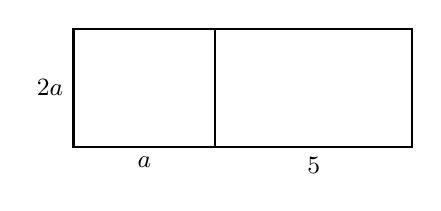
\begin{tikzpicture}[baseline=(current bounding box.center),line width=0.8pt]
\draw (0,0) rectangle (1.8,1.5); \draw (1.8,0) rectangle (4.3,1.5);
\node[left,font=\small] at (0,0.75) {$2a$};
\node[below,font=\small] at (0.9,0) {$a$};
\node[below,font=\small] at (3.05,0) {$5$};
\end{tikzpicture}}{Summe: & \underline{\hspace{4.5cm}} \\[8mm]
Produkt: & \underline{\hspace{4.5cm}}}
\begin{kette}
% NEU
\rk{4x \cdot (a + b) - 3y \cdot (a + b)}{(a + b) \cdot (4x - 3y)}
% NEU
\rk{\frac{3}{4}x^2y - \frac{1}{4}xy^2 + \frac{1}{2}xy}{\frac{1}{4}xy \cdot (3x - y + 2)}
\end{kette}
\end{nr}

\begin{nr}{Gemischt – klammere aus oder löse auf.}
\begin{kette}
% NEU
\rk{14ab - 21b}{7b \cdot (2a - 3)}
% NEU
\rk{3a \cdot (2a - 5)}{6a^2 - 15a}
% NEU
\rk{8x - 2 \cdot (3x - 4)}{2x + 8 = 2 \cdot (x + 4)}
\end{kette}
% terme-e4-k2-s8-v1
% pruef: 0.1*40 + 0.1*25 == 6.5
% pruef: 0.1*(40 + 25) == 6.5
\rs{Eine Hose kostet 40 €, ein Hemd 25 €. Es gibt 10 \% Rabatt. Anna rechnet den Rabatt mit $0{,}1 \cdot 40 + 0{,}1 \cdot 25$, Ben mit $0{,}1 \cdot (40 + 25)$. Begründe, ob beide Terme denselben Rabatt ergeben, und berechne den Rabatt.}{Ja, ausgeklammert ist es derselbe Term; 6,50 €}
\end{nr}

% =================================================================== Einheit 1
\einheit{Terme aufstellen und berechnen}

\begin{nr}{Kannst du das rechnen? Wenn ja, weiter bei Aufgabe \ref{e1p}.}
% NEU
% pruef: 3*Rational(-1,2)**2 - 2*Rational(-1,2) == Rational(7,4)
\rt{Berechne den Wert von $3x^2 - 2x$ für $x = -\frac{1}{2}$.}{$\frac{7}{4}$}
% NEU
% pruef: 3*(5*x - 3) == 15*x - 9
\rt{Die Differenz aus dem Fünffachen einer Zahl $x$ und 3 wird verdreifacht.}{$3 \cdot (5x - 3)$}
\end{nr}

\begin{nr}[b]{Termwerte berechnen – setze ein und rechne.}
\begin{werte}
% terme-e1-k2-s1-v1
\rw{4x - 3}{x = 5}{17}
% terme-e1-k2-s1-v2
\rw{2x + 9}{x = -3}{3}
% terme-e1-k2-s1-v3
\rw{10 - 3x}{x = -2}{16}
% NEU
\rw{x^2 - 4x}{x = -3}{21}
% NEU
\rw{\frac{1}{2}a - 3b}{a = 6,\ b = -\frac{2}{3}}{5}
% NEU
\rw{2 \cdot (x - y)^2 - xy}{x = -1,\ y = 2}{20}
\end{werte}
\end{nr}

\begin{nr}{Terme aufstellen – schreibe einen Term.}
% terme-e1-k1-s2-v2
% pruef: 2*x - 5 == 2*x - 5
\rt{Das Doppelte einer Zahl $x$ wird um 5 vermindert.}{$2x - 5$}
% terme-e1-k1-s4-v1
% pruef: 4*a + 3*b == 4*a + 3*b
\rt{Ein Heft kostet $a$ Euro, ein Stift $b$ Euro. Lena kauft 4 Hefte und 3 Stifte. Was zahlt sie?}{$4a + 3b$}
% GEÄNDERT terme-e1-k1-s3-v3 (Form: Feld neben der Figur)
% pruef: 2*x + 14 == x + 7 + x + 7
\rtx{Umfang des Rechtecks (Maße in cm):}{$2x + 14$}
\figurfelder{\rechteck[seiten={7,x,,},punkte=]{3.2}{1.1}}{& \underline{\hspace{4cm}}}
% terme-e1-k1-s6-v2
% pruef: 5*(4*x - 1) == 20*x - 5
\rt{Nimm das Vierfache einer Zahl $x$, subtrahiere 1 und multipliziere die Differenz mit 5.}{$5 \cdot (4x - 1)$}
\end{nr}

\begin{nr}{Wie in der Prüfung}\label{e1p}
% terme-e1-k1-s7-v1
\par\vspace{4pt}\noindent\makebox[1.6em]{}\lsgt{$2 \cdot (3x - 7)$}%
\parbox[t]{\dimexpr\linewidth-1.6em-\kennbreite\relax}{\raggedright Die Differenz aus dem Dreifachen einer Zahl $x$ und 7 wird verdoppelt. Kreuze den passenden Term an.}%
\parbox[t]{\kennbreite}{\raggedleft\footnotesize P10 ’23}\par
\kreuzzeile{\kreuz{$(3x - 7) : 2$}\kreuz{$3x : 7 \cdot 2$}\kreuz{$2 \cdot (3x - 7)$}\kreuz{$3x - 7 \cdot 2$}}
\end{nr}

\begin{nr}{Für Schnelle}
% NEU
% pruef: 3*x*2 + x*x == 6*x + x**2
% pruef: 3*x + 2 + 2*x + x + x + (2 + x) == 8*x + 4
\rtx{Die Figur besteht aus zwei Rechtecken (Maße in cm). Gib Terme für den Flächeninhalt und den Umfang an und fasse sie zusammen.}{Fläche: $x^2 + 6x$; Umfang: $8x + 4$}
\figurfelder{\begin{tikzpicture}[baseline=(current bounding box.center),line width=0.8pt]
\draw (0,0) -- (4.2,0) -- (4.2,1.0) -- (1.4,1.0) -- (1.4,2.4) -- (0,2.4) -- cycle;
\draw[line width=0.4pt] (0,1.0) -- (1.4,1.0);
\node[below,font=\small] at (2.1,0) {$3x$};
\node[right,font=\small] at (4.2,0.5) {$2$};
\node[above,font=\small] at (0.7,2.4) {$x$};
\node[left,font=\small] at (0,1.7) {$x$};
\end{tikzpicture}}{Flächeninhalt: & \underline{\hspace{4cm}} \\[8mm]
Umfang: & \underline{\hspace{4cm}}}
% NEU
% pruef: 3*(x + x - 3) == 6*x - 9
\rt{Lea ist $x$ Jahre alt, ihr Bruder ist 3 Jahre jünger. Die Mutter ist dreimal so alt wie beide zusammen. Wie alt ist die Mutter?}{$3 \cdot (x + x - 3) = 6x - 9$}
\end{nr}

\begin{nr}{Gemischt}
% NEU
% pruef: 5 - 2*Rational(-3,2)**2 == Rational(1,2)
\rt{Berechne den Wert von $5 - 2x^2$ für $x = -1{,}5$.}{$0{,}5$}
% NEU
% pruef: 3*(x + 4) == 3*x + 12
\rt{Schreibe als Term: das Dreifache der Summe aus einer Zahl $x$ und 4.}{$3 \cdot (x + 4)$}
% terme-e1-k4-s4-v2
% pruef: 4.5 + 2.5*9 == 27
\rs{Ein Taxi kostet 4,50 € Grundpreis und 2,50 € je Kilometer. Stelle einen Term für den Fahrpreis in Euro bei $d$ Kilometern auf. Reichen 25 € für eine Fahrt von 9 km?}{$4{,}50 + 2{,}50d$; nein, 27 €}
\end{nr}

% =================================================================== Lösungen
\clearpage
\noindent{\Large\bfseries Lösungen}\par\vspace{1.5mm}
\noindent\rule{\textwidth}{0.6pt}\par\vspace{2pt}
\begin{multicols}{2}\raggedright\small\linespread{0.96}\selectfont
\mblsg
\end{multicols}
\end{document}
